% PREAMBLE
%%%%%%%%%%%%%%%%%%%%%%%%%%%%%%%%%%%%%%%%%%%%%%%%%%%%%%%%%%%%%%%%%%%%%%%%%%%%%%%%%%%%%%%%%%%%%%%%%%%%%%%%
%%%%%%%%%%%%%%%%%%%%%%%%%%%%%%%%%%%%%%%%%%%%%%%%%%%%%%%%%%%%%%%%%%%%%%%%%%%%%%%%%%%%%%%%%%%%%%%%%%%%%%%%
\documentclass[10pt]{article}
\usepackage{geometry}                	% See geometry.pdf to learn the layout options. There are lots.
\geometry{top=1.0in, bottom=1.0in, left=1.0in, right=1.0in}                   	% ... or a4paper or a5paper or ...
%\geometry{landscape}                	% Activate for for rotated page geometry
\usepackage{fancyhdr} 			% This should be set AFTER setting up the page geometry
\pagestyle{fancy} 				% options: empty , plain , fancy
\renewcommand{\headrulewidth}{0pt} % customise the layout...
\lhead{}\chead{}\rhead{}
\lfoot{}\cfoot{\thepage}\rfoot{}
%\usepackage[parfill]{parskip}   	   	% Activate to begin paragraphs with an empty line rather than an indent
\usepackage{graphicx}
\usepackage{amssymb}
\usepackage{epstopdf}
\usepackage{booktabs} 			% for much better looking tables
\usepackage{array} 				% for better arrays (eg matrices) in maths
\usepackage{paralist} 			% very flexible & customisable lists (eg. enumerate/itemize, etc.)
\usepackage{verbatim}			% adds environment for commenting out blocks of text & for better verbatim
\usepackage{subfigure} 			% make it possible to include more than one captioned figure/table in a single float
\usepackage{algorithmic}
\DeclareGraphicsRule{.tif}{png}{.png}{`convert #1 `dirname #1`/`basename #1 .tif`.png}
\usepackage{sectsty}
%\allsectionsfont{\sffamily\mdseries\upshape} 	% (See the fntguide.pdf for font help)
%\usepackage[utf8]{inputenc} 		% Any characters can be typed directly from the keyboard, eg éçñ
%\usepackage{textcomp} 		% provide lots of new symbols
\usepackage{graphicx}  			% Add graphics capabilities
\usepackage{epstopdf} 			% to include .eps graphics files with pdfLaTeX
\usepackage{flafter}  			% Don't place floats before their definition
\usepackage{amsmath,amssymb} 	% Better maths support & more symbols
\usepackage{bm}  				% Define \bm{} to use bold math fonts
\usepackage{memhfixc}  			% remove conflict between the memoir class & hyperref
%\usepackage{pdfsync}  			% enable tex source and pdf output syncronicity
\usepackage[pdftex,bookmarks,colorlinks,breaklinks]{hyperref}  % PDF hyperlinks, with coloured links
\hypersetup{linkcolor=black,citecolor=black,filecolor=black,urlcolor=black} % black links, for printed output
\usepackage{cite}
\usepackage{mathtools}
\usepackage{subfigure}			% for putting figures "side-by-side"
%\usepackage{sidecap}			% sidecaption figures
\usepackage{wrapfig}
\usepackage{caption}
\usepackage{multicol}

%\makeatletter
%\newenvironment{tablehere}
  %{\def\@captype{table}}
  %{}

%\newenvironment{figurehere}
 % {\def\@captype{figure}}
 % {}
%\makeatother


% Title Page
\title{\textbf{CBEMD} Parallelized Molecular Dynamics in Various Thermodynamic Ensembles}
\author{Nathan A. Mahynski, George A. Khoury, Carmeline J. Dsilva, \\
Arun Prabhu, Francesco Ricci, and Junyoung Park}
\date{}

\begin{document}
\maketitle
\begin{figure}[htbp]
   \centering
   
\includegraphics[width=2.5in]{princeton.jpg}
\end{figure}
\thispagestyle{empty}
\newpage
\setcounter{page}{1}
\pagenumbering{arabic}
\newpage

\section{Introduction}
We propose to develop a software package to perform parallelized molecular dynamics (MD) calculations for several different thermodynamic ensembles. 
%
Molecular dynamics is a technique commonly used to simulate the motions of a system of interest on a microscopic level; one can then calculate macroscopic properties from the microscopic features of this system. 
%
Properties such as diffusion coefficients, specific heats, and chemical potentials, which are often difficult or impossible to measure in experiment, are commonly calculated in MD.  
%
Because of the myriad of properties that can be calculated, MD has applications such fields as material science, pharmaceutical design, cellular biology, thermodynamics, and fluid mechanics.  
%
Due to its relative simplicity and its ability to be massively parallelized, MD is a common but powerful tool for many scientists and engineers today.

\section{Background on Molecular Dynamics}
MD first initializes a system of particles, usually thought of as atoms, molecules, or another relevant (molecular-scale) group.  
%
Given an interaction potential $V (\overrightarrow{r})$ between these particles, MD integrates Newton's equation of motion, $\overrightarrow{F}=m\overrightarrow{a}$, forward in time.  
%
Thus, the flow of the program follows a well defined set of steps:
\begin{enumerate}
    \item Initialize positions and choose a timestep, $dt$
    \item Calculate the forces $\overrightarrow{F} =  -\nabla V (\overrightarrow{r}) $
    \item Numerically integrate to calculate the displacement over $dt$, using the relationships $\overrightarrow{F}=m\overrightarrow{a}$, $\overrightarrow{a} = \frac{\overrightarrow{dv}}{dt}$, and $\overrightarrow{v} = \frac{\overrightarrow{dr}}{dt}$
    \item Update positions and time
    \item Repeat from step 2 until final time
\end{enumerate}

Users of any molecular dynamics program must provide the initial configuration for the particles.  
%
The user must also supply the relevant potential function $V$. Different potential functions can be used to describe the system at different levels of accuracy. 
%
These functions typically try to capture van der Waals interactions due to coupling of electron clouds, but can also incorporate additional effects, such as long range charge-charge interactions and solvation interactions (Debye screening effects). 
%
Our project will provide an easily extensible interface so that the user can incorporate additional interactions.

For numerical stability, the timestep $dt$ is typically on the order of a femtosecond. 
%
The longest simulations reported for macromolecules such as proteins are on the microsecond timescale, but such lengthy simulations can require specialized supercomputing hardware such as ANTON or GPUs. 
%
Although the time integration must be done sequentially, at each step, the evaluation of the potential energy and forces can be parallelized, which is the primary reason MD has been so successful on large computer clusters.

There are many different numerical integration algorithms that have been developed, each with a slightly different purpose and numerical stability.  
%
In this project, we implemented the Verlet integrator and the Andersen thermostat.
%
Both of these integration schemes are developed specifically for molecular dynamics.

Several existing MD packages, such as HOOMD, LAMMPS, GROMACS, and NAMD, incorporate such ensembles. Members of our group use some of these codes in our every day research, but we do not know much about their internal structure. Therefore, it was a prudent exercise to develop our own codebase with a well-written interface that we can each extend for our custom applications.

\subsection{Verlet integrator}
The Verlet integrator is designed to maintain constant energy ($E$), volume ($V$), and number of particles ($N$).  
%
This NVE ensemble is known in thermodynamics as the {\em microcanonical ensemble}.

The Verlet integrator equations are
$$ \overrightarrow{r}(t + \Delta t) = 2 \overrightarrow{r}(t) - \overrightarrow{r}(t- \Delta t) + \frac{\overrightarrow{F}(t) \Delta t ^2}{m}$$

$$ \overrightarrow{v}(t + \Delta t) = \frac{\overrightarrow{r}(t + \Delta t) - \overrightarrow{r}(t)} {\Delta t} $$

These equations can be used to update the positions and velocities of the atoms in the system, given the current positions and forces on the atoms.

\subsection{Andersen thermostat}
The Andersen thermostat is designed to maintain constant temperature ($T$), volume ($V$), and number of particles ($N$).  
%
This NVT ensemble is known in thermodynamics as the {\em canonical ensemble}.

The Andersen thermotat equations are

\section{Code Goals and Structure}
Our code was written with the goals of generalizability and efficiency.

Our code is written in C++, and utilizes many object-oriented features. 
%
The modular class structure allows for a general coding framework, such that users can easily define their own intergrators, pair potentials, and bond types. 
%
We have parallelized our code using MPI. 
%

We have defined various classes for the different parts of our MD simulation. 
%
\begin{enumerate}
\item Atom: The atom class contains only an atom structure. This structure is passed between processors when the code is run in parallel.
\item Integrator: The integrator class is an abstract base class. It defines the implementation structure for integrators. We have implemented two integrators (Verlet and Andersen), but our code can easily be extended to other integration schemes. 
\item Interaction: The interaction class is an abstract base class. It defines the interaction between two atoms, including a function pointer to different interaction potentials. We have implemented standard Lennard-Jones potential, the harmonic bond potential, and the finitely extensiable nonlinear elastic (fene) bond potential. 
\item System: The system class stores the information for the total simulation, including the box size, a list of atoms, and the interactions between atoms (stored as a matrix of function pointers to different interactions). When the code is run in parallel, each processor contains a system object that contains the atoms owned by that processor.
\end{enumerate}

We also have files ``read\_interaction.cpp'' and ``read\_xml.cpp'', which handle file I/O. 
%

The flow of our code is as follows:
\begin{enumerate}
\item The code reads in the starting configuration from the user-supplied xml file, and the relevant energy parameters from the user-supplied energy file. Atoms are read from the xml file and assigned to the correct processor. 
\item A system is initialized for each processor containing the relvant system parameters from the xml file.
\item An integrator is initialized on each processor. 
\item The forces on each atom are calculated
\item When the code is run in parallel, the ``ghost'' atoms near the edges of each processor domain are passed to the relevant neighboring processor, and the forces between these ghost atoms and the atoms owned by the processor are calculated
\item The atomic positions are updated via the ``step()'' function for the instantiated integrator
\item Any atoms that have moved outside of the processor domain are passed to the relevant processor.
\end{enumerate}
Steps 4-8 are repeated for each timestep. 
%
At each time step, the configuration of the system is output to a file.
%
This output file can be read by VMD, a molecular visualization package.

\subsection{Input and Output}
Our code is initialized using user-supplied xml and energy files.
%
The xml file contains information such as the positions, velocities, and masses of all the atoms in the simulation.
%
%%%ADD SAMPLE FILE/FILE FORMAT
%
The energy file contains the parameters for each interaction type in the xml file.
%%%ADD SAMPLE
%
At each timestep, our code writes the current configuration to an output file in ``xyz'' format. 
%
This file contains the positions of every atom in the simulation, and the ``xyz'' format is easily read by VMD and other molecular visualization packages.

To parse the xml file, we used the Boost C++ library to allow for discrepancies in the xml file (such as extra white space, input arguments in arbitrairy orders, etc.).

\subsection{Domain decomposition}
In the final version of our code, we utilize a one-dimensional domain decomposition, where the simulation box is decomposed into vertical slabs.
%
Each vertical slab and the atoms it contains are assigned to a processor, and atoms are passed between processors as needed using MPI. 
%
However, we began our project with attempting a three-dimensional domain decomposition.
%
Although we could not get this algorithm completely debugged by the end of this project, we will include information on the structure and implementation since it comprised a large part of our efforts.

The 3-D domain decomposition attempts to spatially split the simulation box into a number of
identical domains based on the number of processors available. Each processor will then be responsible
for one domain. Parallelization will be most efficient if each processor has approximately the same load.
If we assume that the particles are uniformly distributed in the simulation box, then the most efficient
way to partition the system is one in which the individual domains are as cubic as possible. This is what
the 3-D domain decomposition algorithm attempts to do.

Note: The 3-D domain decomposition assumes that the simulation box is a rectangular parallelepiped
with one corner positioned at (0,0,0).

The algorithm is as below
\begin{enumerate}
\item Generate the prime factorization of the number of processors available (e.g. $36 = 2 \times 2 \times 3 \times 3$).
\item Generate a set of 3 numbers by combining the factors in different ways such that the product
is still the number of processors available (e.g. for the case of 36 processors, possible sets are
$\{2,3,6\}, \{3,2,6\}, \{1,4,9\}, \{2, 1, 18\}$, etc.).
\item Divide the simulation box into domains by dividing the $x$, $y$, $z$ directions respectively into a
number of parts based on the 3 numbers in one of the sets generated in step 2. (See Fig. \ref{fig:ddecomp} for an
example)
\item Check how cubic the domains are by evaluating $diff = (d_1-d_2)^2+(d_2-d_3)^2+(d_3-d_1)^2$ ; where $d_1$, $d_2$, $d_3$
are the $x$, $y$, $z$ dimensions of a domain (since all the domains are the same size and shape).
\item Repeat steps 3-4 for all the sets generated in step 2 while keeping track of the set that resulted
in the smallest value of diff.
\item Divide the simulation box into domains based on the set which generated the smallest value of
diff.
\item Assign the domains to processors by stepping through each domain in the $x$-direction from
lowest to highest and then in $y$ and then in $z$. (See Fig. \ref{fig:ddecomp} for an example)
\end{enumerate}

The code implements steps 2-4 through the recursive function gen\_sets in domain\_decomp.cpp.
The function init\_domain\_decomp in domain\_decomp.cpp starts the process from step 1 through 6
calling gen\_sets along the way.

\begin{figure}[htb]
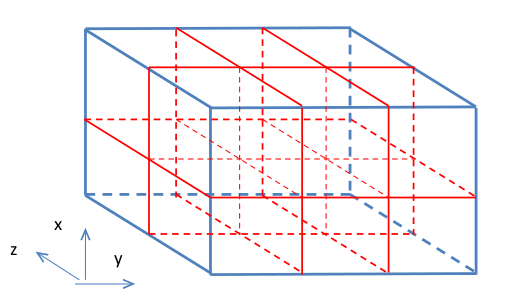
\includegraphics[width=0.5\textwidth]{ddecomp.jpg}
\caption{An example of the domain decomposition. The set in use is $\{2,3,2\}$ (see step 3 of the algorithm).}
\label{fig:ddecomp}
\end{figure}

\section{Validation}
We have compared the results of our code to LAMMPS, a molecular dynamics software package.
%
The comparison is shown in Figure ??.

\section{Profiling Results}
We used gprof to profile our code and highlight the computational bottlenecks.

\section{Optimization}
From the results of our profiling, we opted to optimize the ``min\_image\_dist2()'' and the ``slj()'' functions.

The ``min\_image\_dist2()'' uses the ``round'' function from the math library. 
%
For dense systems, or for short simulations, this is inefficient, because most atoms are still near each other.
%
Therefore, we replaced the ``round'' function with a while loop that adjusts the distance until it is the minimum image distance.

The ``slj()'' function uses the ``pow'' function from the math library to compute $r^6$.
%
However, this function call is probably expensive and could be replaced by $r \times r \times r \times r \times r \times r$.
%

\section{Scaling}
We looked at how the execution time of our code scaled with the number of processors.

\section{Conclusion}



\end{document}
